\section{Introduction}\label{sec:intro}

\begin{figure*}
    \centering
    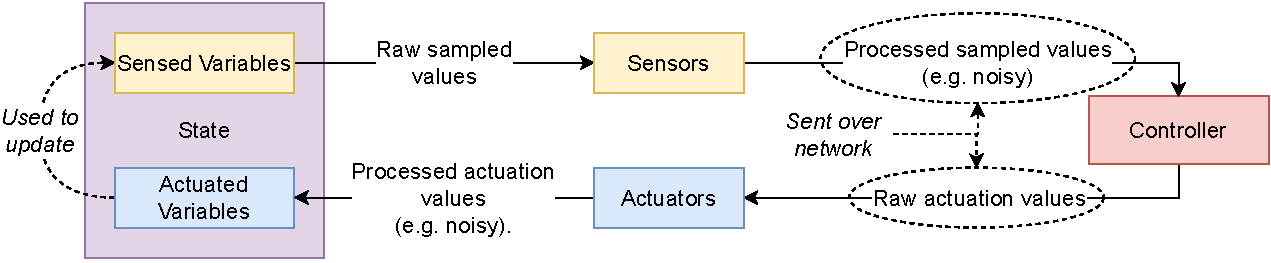
\includegraphics[width=.8\textwidth]{CLEAVE_NCS_structure}
    \caption{
        Structure of an emulated \ac{NCS} in \ac{CLEAVE}.
    }\label{fig:cleave:ncs:struct}
\end{figure*}

The number and applications of \acp{CPS}~\cite{Rajkumar2010CPS} --- i.e.\ systems in which a real, physical mechanism is controlled by a computer --- have exploded in recent years.
However, this rapid increase in adoption has mostly been limited to industrial contexts.
Although \acp{CPS} present huge opportunities for all facets of society, they have yet to reach our daily lives in any relevant scale due to their stringent operational requirements.
This is about to change, however, as with the advent of novel wireless communication technologies as well as networking paradigms, such as cellular 5G and Edge Computing~\cite{Satya2017Emergence}, consumer-grade \acp{CPS} will be made possible.
These technologies meet two key requirements of \acp{CPS}: real-time capabilities (through extremely low end-to-end latencies), and context- and locality-awareness, and will most likely become the backbone of \ac{CPS} in the future.

A subcategory of \acp{CPS} which stands to particularly benefit from the adoption of the above technologies is \acp{NCS}~\cite{Gupta2010NCSOverview}, a type of \ac{CPS} wherein multiple networked actuators and sensors form a part of the same automatic control system.
Depending on the physical system being controlled, \acp{NCS} can have stringent timing and reliability requirements for the communication between components that conventional cloud paradigms and cellular networks are unable to meet~\cite{Wan2020Efficient}.

Due to their potential advantages for industrial and commercial settings, a large body of work exists dedicated to the modelling and performance characterization of \acp{NCS}~\cite{Zhang2013Survey,Zhang2016Survey}.
They improve and flexibilize existing control systems by allowing for the distribution of control functions over and across networks.
This allows for, e.g.\ centralized coordination, control, and monitoring of potentially hundreds of devices.

Most of the large literature concerning \acp{NCS}, however, follows a theoretical approach, and only a small fraction of it deals with experimental studies.
The inherent inter-domain nature of \acp{NCS}, which intertwines knowledge from the fields of communications, computing, and control theory, coupled with the complexity of experimental platforms make these kinds of studies hard to perform.

One approach to experimental research in \acp{NCS} uses setups in which the complete system is built on top of real hardware.
This approach is employed in the works of, for instance, \textcite{Li2014Wireless,Baumann2018LowPower,Cuenca2019UAV}; in all of these, the authors implement and validate their results on physical testbeds.
Conversely, other studies choose to instead use completely \emph{simulated} \ac{NCS} setups.
\textcite{Wu2012NPC,Chen2015synccontrol,Ma2019DynamicSched} are examples of works in which the authors have opted for such completely virtualized approaches.
These studies often employ combinations of physical and network simulation tools to try to capture the complex dynamics of \acp{NCS}.
Finally, a number of experimental studies instead employ \emph{virtualized} approaches, in which either
\begin{enumerate*}[itemjoin={{; }}, itemjoin*={{; or }}]
    \item a real network interacts with a simulated or emulated control system~\cite{Wang2020VoltageControl}
    \item an emulated or simulated network interacts with a real control system~\cite{Natale2004InvPendEthernet}.
\end{enumerate*}

As evidenced above, experimental research in \acp{NCS} includes a large variety of heterogeneous hardware and software platforms, as well as methodologies and \aclp*{KPI}.
This, in turn, leads to hardware, software, and methodology fragmentation, as different studies tend to prefer approaches more favored in their respective communities.
Furthermore, existing studies tend to focus on individual aspects and components of a system, thus producing results which do not provide a complete image of the \ac{NCS}.
This has caused a gap in knowledge pertaining to the reproducibility and comparison of experimental studies on these systems.

\textcite{Zoppi2020NCSBench} made the first (and to the best of our knowledge, the only) attempt at tackling this challenge with their \emph{NCSbench} platform.
\emph{NCSbench} is an open-source \ac{NCS} benchmarking platform, built on top of the LEGO\textregistered{}\ Mindstorms EV3 Core Set\texttrademark{}\ platform, with stated goals of reproducibility and ease of use.
It achieves this thanks to its low-cost, accessibility, and ease of reconfiguration.

Although \emph{NCSbench}~\cite{Zoppi2020NCSBench} is a relevant and important step towards the reproducibility of \ac{NCS} benchmarks, we believe it still falls short on some aspects.
In particular, we argue the reliance of the tool on specific hardware for the Plant hampers the potential of the platform.
The LEGO Mindstorms platform, although accessible and flexible, still fundamentally limits the physical systems that can be benchmarked to the kind of systems that can be physically implemented on it.
Furthermore, it is \emph{not} scalable, and thus unsuitable for studies of larger, distributed \acp{NCS}.

In this paper, we present the first fully-software-based framework for scalable and repeatable benchmarking of edge-native \ac{NCS}.
As the Edge computing paradigm starts to be adopted by industry, more and more variations of it have started to appear in literature.
``Near'', ``far'', ``core'', and ``telco'' edge, among others, are all terms which describe variations of the original concept and which are becoming ubiquitous in new research.
While the core idea of Edge computing is widely accepted as fundamental for pervasive \acp{NCS} in general, understanding the strenghts and weaknesses of such different edge concepts is of paramount importance.

Our framework, which we name \ac{CLEAVE}, aims to simplify the repeatable and scalable benchmarking of such systems. 
It is built on top of the \emph{Python 3.8} language, making it highly extensible and able to harness the hundreds-of-thousands of already existing user-provided libraries and packages.
Additionally, it is compatible with \emph{containerization} technologies such as \emph{Docker}\footnote{Docker Engine: \url{https://www.docker.com/}}, making it suitable for automated deployment and benchmarking on industry-standard cloud and (more importantly) edge setups using container orchestration technologies.

The rest of this paper is structured as follows.
\cref{sec:approach} presents the design principles of the framework.
In \cref{sec:experiments}, we present a series of experiments which validate the utility, flexibility, and repeatability of \ac{CLEAVE}.
Finally, in \cref{sec:conclusion} we conclude this paper and briefly discuss future work.